\documentclass[12pt]{article}

\usepackage[utf8]{inputenc}
\usepackage[T1]{fontenc}
% babel not required; document is in Portuguese
\usepackage{times}
\usepackage[a4paper,top=3.5cm,left=3.0cm,right=3.0cm,bottom=2.5cm]{geometry}
\usepackage{graphicx}
\usepackage{booktabs}
\usepackage{amsmath,amssymb}
\usepackage{listings}
\usepackage{xcolor}
\usepackage{hyperref}
\usepackage{pgfplots}
\pgfplotsset{compat=1.18}
\usepackage{float}
\usepackage{caption}
\usepackage{enumitem}
\usepackage{multicol}
\usepackage{titlesec}
\usepackage{abstract}

% ---- SBC-like formatting ----
\setlength{\parindent}{0pt}
\setlength{\parskip}{5pt}

% List formatting
\setlist{leftmargin=1.5em, itemsep=2pt, topsep=4pt, parsep=0pt}
\setlist[enumerate]{label=\arabic*.}
\setlength{\columnsep}{0.8cm}

% Section formatting SBC style
\titleformat{\section}{\normalfont\bfseries\normalsize}{\thesection.}{0.5em}{}
\titleformat{\subsection}{\normalfont\bfseries\normalsize}{\thesubsection.}{0.5em}{}
\titlespacing{\section}{0pt}{12pt plus 2pt minus 1pt}{4pt plus 1pt minus 1pt}
\titlespacing{\subsection}{0pt}{8pt plus 2pt minus 1pt}{4pt plus 1pt minus 1pt}

% Abstract formatting
\renewenvironment{abstract}{%
  \small\begin{center}\bfseries Resumo\end{center}%
  \begin{quotation}\noindent
}{%
  \end{quotation}
}

\hypersetup{
  colorlinks=true,
  linkcolor=blue!60!black,
  urlcolor=blue!60!black,
  citecolor=blue!60!black
}

\definecolor{codegray}{rgb}{0.95,0.95,0.95}
\lstset{
    basicstyle=\ttfamily\footnotesize,
    backgroundcolor=\color{codegray},
    breaklines=true,
    frame=single,
    framerule=0pt,
    xleftmargin=0.5em,
    xrightmargin=0.5em,
    showstringspaces=false,
    keywordstyle=\color{blue!60!black}\bfseries,
    commentstyle=\color{green!40!black}\itshape,
    stringstyle=\color{red!50!black},
    language=Java
}

% Allow flexible line breaking to avoid overfull hboxes
\sloppy
\setlength{\emergencystretch}{2em}

% ---- Title ----
\title{\textbf{TP01 -- Pontes e Caminho Euleriano}\\[0.3em]
\large Métodos Naïve e Tarjan + Algoritmo de Fleury}

\author{
Diego Henrique Xavier dos Santos \\
Marcos Vinícius Nunes Reis \\
Vitor Daniel Silva Melo \\[0.4em]
\small PUC Minas -- Ciência da Computação \\
\small Teoria dos Grafos e Computabilidade \\
\small Prof. Zenilton Kleber Gonçalves do Patrocínio Júnior
}

\date{}

% ====================================================================
\begin{document}
% ====================================================================

\maketitle

% ---- Resumo ----
\begin{abstract}
Este trabalho apresenta a implementação e comparação de dois métodos de
identificação de pontes em grafos --- o \textbf{método naïve}
(custo $O(E \cdot (V{+}E))$) e o \textbf{método de Tarjan}
(custo $O(V{+}E)$) --- acoplados ao \textbf{Algoritmo de Fleury}
para construção de caminhos eulerianos. Experimentos com grafos de 100 a
100.000 vértices revelam que o Tarjan é até $108\times$ mais rápido na
enumeração de pontes, mas o naïve, com otimização \textit{isReachable},
supera o Tarjan no contexto do Fleury para grafos esparsos de tamanho
médio --- resultado contraintuitivo explicado pelo custo real de cada
chamada a \textit{isBridge}.
\end{abstract}

\vspace{1em}
\hrule
\vspace{1.5em}

% ====================================================================
\section{Introdução}
% ====================================================================

Uma \textbf{ponte} é uma aresta cuja remoção desconecta o grafo. O conceito
aparece em inúmeros problemas práticos --- detecção de pontos críticos em
redes de comunicação, planejamento de rotas e, em particular, a construção
de \textbf{caminhos eulerianos}: sequências que percorrem cada aresta do
grafo exatamente uma vez.

O algoritmo de Fleury, que constrói esses caminhos, precisa a cada passo
decidir se uma aresta candidata é ponte. A estratégia escolhida para essa
decisão muda profundamente o comportamento prático do algoritmo.

Neste trabalho implementamos dois métodos de identificação de pontes:
\begin{enumerate}
    \item \textbf{Método naïve}: para cada aresta $(u,v)$, remove-a, testa
          conectividade via DFS/BFS e a reinsere. Custo $O(E \cdot (V{+}E))$.
    \item \textbf{Método de Tarjan (1974)}: uma única DFS calculando valores
          \textit{disc} e \textit{low}. Custo $O(V{+}E)$.
\end{enumerate}

Ambos são acoplados ao Fleury por meio de uma interface comum
(\textit{Strategy Pattern}), permitindo trocar a estratégia sem alterar o
restante do código. Por fim, comparamos o tempo médio das duas abordagens em
grafos aleatórios de $100$, $1.000$, $10.000$ e $100.000$ vértices, nos três
tipos eulerianos exigidos pelo enunciado.

% ====================================================================
\section{Fundamentos Teóricos}
% ====================================================================

\subsection{Grafos e definições básicas}

Um \textbf{grafo simples não-direcionado} $G = (V, E)$ é composto por um
conjunto de vértices $V$ e um conjunto de arestas
$E \subseteq \binom{V}{2}$, sem laços nem arestas paralelas. O
\textbf{grau} $\deg(v)$ de um vértice $v$ é o número de arestas incidentes
a ele.

\textbf{Lema do aperto de mão (\textit{Handshaking Lemma}):} em qualquer
grafo, $\sum_{v \in V} \deg(v) = 2|E|$, portanto o número de vértices de
grau ímpar é sempre par.

\subsection{Quando existe caminho ou circuito euleriano}

Pelo \textbf{Teorema de Euler}, num grafo conexo:
\begin{itemize}
    \item existe \textbf{circuito euleriano} se e somente se todos os
          vértices têm grau par;
    \item existe \textbf{caminho euleriano} (sem ser circuito) se e somente
          se exatamente dois vértices têm grau ímpar (esses dois serão os
          extremos do caminho);
    \item caso contrário, nem caminho nem circuito existem.
\end{itemize}

Essa classificação é o primeiro passo do Fleury: se o grafo for
não-euleriano, o algoritmo aborta imediatamente sem percorrer nenhuma
aresta.

\subsection{Pontes e método naïve}

\begin{quote}
\textbf{Definição.} Uma aresta $(u,v) \in E$ é uma \textit{ponte} se o
grafo $G - (u,v)$ tem mais componentes conexas que $G$.
\end{quote}

O método naïve é literalmente a definição codificada. Para cada aresta
$(u,v)$:
\begin{enumerate}
    \item Remove $(u,v)$ do grafo.
    \item Verifica se $v$ ainda é alcançável a partir de $u$ (DFS/BFS).
    \item Reinsere $(u,v)$.
    \item Se a resposta foi ``não'', $(u,v)$ é ponte.
\end{enumerate}

Custo: $O(E \cdot (V{+}E))$ --- uma DFS por aresta.

\textbf{Otimização implementada:} em vez de \texttt{isConnected()} ---
que varre todo o grafo --- usamos \texttt{isReachable(u,\,v)}, que
interrompe a DFS assim que encontra $v$. Em grafos esparsos essa terminação
antecipada reduz significativamente o tempo prático.

\subsection{Método de Tarjan (1974)}
\label{sec:tarjan}

A ideia central é trocar $E$ travessias independentes por uma única DFS.
Durante a passagem, mantemos para cada vértice $v$ dois valores:
\begin{itemize}
    \item $\mathrm{disc}(v)$: instante de descoberta de $v$ na DFS
          (contador global incrementado a cada visita);
    \item $\mathrm{low}(v)$: o menor $\mathrm{disc}$ alcançável a partir
          da subárvore de $v$ usando zero ou mais arestas da árvore DFS
          seguidas de \emph{no máximo uma} aresta de retorno
          (\textit{back-edge}).
\end{itemize}

A atualização é:
\[
\mathrm{low}(v) = \min\!\Big(\mathrm{disc}(v),\;
    \min_{(v,w) \in \text{back-edges}} \!\mathrm{disc}(w),\;
    \min_{(v,c) \in \text{árvore}} \!\mathrm{low}(c)\Big)
\]

\textbf{Condição de ponte:} a aresta $(u,v)$ --- onde $v$ é filho de $u$
na árvore DFS --- é ponte se e somente se
\[
\mathrm{low}(v) > \mathrm{disc}(u).
\]

Em palavras: nenhum caminho que sai da subárvore de $v$ consegue alcançar
$u$ ou qualquer ancestral de $u$ por outro caminho. Custo: $O(V{+}E)$ ---
uma única DFS.

\textbf{Implementação iterativa:} a versão recursiva existe no código
(\texttt{TarjanBridgeFinderRec.java}) por valor didático, mas não é usada
nos experimentos. Para $V \geq 10.000$, a profundidade da recursão
ultrapassa a pilha padrão da JVM, causando \texttt{StackOverflowError}
mesmo com \texttt{-Xss64m}. A versão iterativa simula a DFS com uma pilha
explícita de inteiros \cite{so-tarjan,so-dfs}, sem esse problema.

\subsection{Algoritmo de Fleury}
\label{sec:fleury}

O Fleury constrói o caminho euleriano percorrendo arestas uma a uma:
\begin{enumerate}
    \item Classifique o grafo; se for não-euleriano, aborte.
    \item Escolha $v_0$: um vértice de grau ímpar (semi-euleriano) ou
          qualquer vértice de grau positivo (euleriano).
    \item Estando em $u$, prefira sempre uma aresta que \textbf{não} seja
          ponte; pontes são último recurso.
    \item Remova a aresta percorrida, mova-se para o vizinho e repita até
          esgotar todas as arestas.
\end{enumerate}

A regra de evitar pontes é o que evita ficar preso: atravessar uma ponte
prematuramente pode isolar arestas que ainda precisariam ser percorridas.
O custo do Fleury é dominado pela detecção de pontes a cada passo:
$O(E \cdot (V{+}E))$ com qualquer das duas estratégias.

% ====================================================================
\section{Implementação}
% ====================================================================

\subsection{Visão geral dos arquivos}

Todo o projeto está em Java~21. A Tabela~\ref{tab:arquivos} resume os
arquivos e suas responsabilidades.

\begin{table}[H]
\centering
\caption{Arquivos do projeto e suas responsabilidades.}
\label{tab:arquivos}
\small
\begin{tabular}{p{5.8cm}p{7.9cm}}
\toprule
Arquivo & Responsabilidade \\
\midrule
\texttt{Graph.java}                 & Lista de adjacência, versão, grau, arestas \\
\texttt{GraphUtils.java}            & DFS, BFS, conectividade, \texttt{isReachable}, classificação euleriana \\
\texttt{GraphGenerator.java}        & Geração de grafos eulerianos, semi e não-eulerianos \\
\texttt{BridgeFinder.java}          & Interface \textit{Strategy} para detecção de pontes \\
\texttt{NaiveBridgeFinder.java}     & Naïve: remove $\to$ \texttt{isReachable} $\to$ reinsere \\
\texttt{TarjanBridgeFinder.java}    & Tarjan iterativo com cache versionado \\
\texttt{\footnotesize TarjanBridgeFinderRec.java} & Tarjan recursivo (didático; não usado nos experimentos) \\
\texttt{FleuryEulerPath.java}       & Fleury parametrizado por \texttt{BridgeFinder} \\
\texttt{Experiments.java}           & Bateria de experimentos $\to$ CSV \\
\texttt{Main.java}                  & Menu interativo com seleção de tamanho e densidade \\
\bottomrule
\end{tabular}
\end{table}

\subsection{Estrutura de dados: lista de adjacência}

Usamos lista de adjacência (\texttt{LinkedList<Integer>[]}). A alternativa,
matriz de adjacência, ocuparia $O(V^2)$ de memória: para $V=100.000$ isso
representa $10^{10}$ posições --- completamente inviável. Lista de
adjacência custa $O(V{+}E)$ e permite remoção e inserção de arestas em
tempo razoável, operações que o naïve realiza em todo par de arestas.

\subsection{Interface comum: BridgeFinder}

A interface \texttt{BridgeFinder} é o ponto de troca de estratégia.
O Fleury não conhece a implementação concreta, apenas pergunta:

\begin{lstlisting}
public interface BridgeFinder {
    List<int[]> findBridges(Graph g);        // enumera todas as pontes
    boolean     isBridge(Graph g, int u, int v); // verifica uma aresta
    String      getName();
}
\end{lstlisting}

Isso segue o \textit{Strategy Pattern}: trocar naïve por Tarjan (ou
vice-versa) não exige nenhuma alteração no Fleury.

\subsection{Otimização: isReachable no método naïve}

Em vez de \texttt{isConnected(g)} --- que percorre todos os $V$ vértices
--- o naïve chama o método
\texttt{GraphUtils\allowbreak.isReachable(\allowbreak g,\,u,\,v)},
uma DFS que interrompe a busca assim que encontra $v$ \cite{so-dfs}:

\begin{lstlisting}
public static boolean isReachable(Graph g, int u, int v) {
    Deque<Integer> stack = new ArrayDeque<>();
    Set<Integer>  visited = new HashSet<>();
    stack.push(u);
    while (!stack.isEmpty()) {
        int cur = stack.pop();
        if (cur == v) return true;      // encontrou, para aqui
        if (visited.contains(cur)) continue;
        visited.add(cur);
        for (int nb : g.getNeighbors(cur))
            if (!visited.contains(nb)) stack.push(nb);
    }
    return false;
}
\end{lstlisting}

Em grafos esparsos (onde a maioria dos vértices tem grau~1 ou~2), $v$ é
encontrado rapidamente e a DFS percorre apenas uma fração do grafo.

\subsection{Cache versionado no Tarjan}

O Fleury chama \texttt{isBridge} várias vezes seguidas no mesmo estado do
grafo (uma vez por vizinho candidato do vértice atual). Recomputar
\texttt{findBridges} --- custo $O(V{+}E)$ --- a cada chamada seria
desperdício.

A solução é um \textbf{cache invalidado por versão}: o \texttt{Graph}
mantém um contador inteiro (\texttt{version}), incrementado a cada
\texttt{addEdge}/\texttt{removeEdge}. O Tarjan armazena o par (versão
observada, conjunto de pontes); se a versão atual for a mesma, retorna o
cache:

\begin{lstlisting}
@Override
public boolean isBridge(Graph g, int u, int v) {
    if (g != cacheGraph || g.getVersion() != cacheVersion) {
        cacheGraph   = g;
        cacheVersion = g.getVersion();
        cacheBridgeKeys = new HashSet<>();
        for (int[] e : findBridges(g))
            cacheBridgeKeys.add(GraphUtils.edgeKey(e[0], e[1]));
    }
    return cacheBridgeKeys.contains(GraphUtils.edgeKey(u, v));
}
\end{lstlisting}

Sem cache, Fleury+Tarjan custaria $O(\deg \cdot E \cdot (V{+}E))$; com
cache, cai para $O(E \cdot (V{+}E))$.

\subsection{Geração de grafos}

O \texttt{GraphGenerator} produz grafos dos três tipos exigidos:
\begin{itemize}
    \item \textbf{Euleriano:} começa com um ciclo hamiltoniano (todos com
          grau~2, já par), adiciona ciclos aleatórios extras e ao final
          corrige eventuais resíduos ímpares emparelhando vértices dois a
          dois.
    \item \textbf{Semi-euleriano:} parte do euleriano e adiciona uma única
          aresta entre dois vértices de grau par, tornando ambos ímpares
          (exatamente~2 vértices ímpares).
    \item \textbf{Não-euleriano:} parte do euleriano e adiciona~2 arestas
          independentes (sem vértice em comum), criando~4 vértices de grau
          ímpar.
    \item \textbf{Genérico conexo:} spanning tree aleatória mais arestas
          extras sorteadas até atingir o número alvo. Usado para testes de
          estrutura e DFS/BFS.
\end{itemize}

% ====================================================================
\section{Experimentos}
% ====================================================================

\subsection{Configuração}

\begin{itemize}
    \item \textbf{Hardware/SO:} Linux x86\_64.
    \item \textbf{JDK:} OpenJDK~21; JVM com flags \texttt{-Xss64m -Xmx2g}.
    \item \textbf{Repetições:} 3 execuções por configuração; reportamos a
          média.
    \item \textbf{Tamanhos:} $N \in \{100,\; 1.000,\; 10.000,\; 100.000\}$.
    \item \textbf{Densidade:} aproximadamente $1{,}1 \cdot V$ arestas
          (grafo esparso, próximo de uma árvore com poucas arestas extras).
    \item \textbf{Tipos:} Euleriano, Semi-euleriano e Não-euleriano.
    \item \textbf{Marcação ``--'':} configuração pulada porque a estimativa
          de tempo ultrapassava~5 minutos por execução.
\end{itemize}

\subsection{Tempo médio para encontrar todas as pontes}

\begin{table}[H]
\centering
\caption{Tempo médio de \texttt{findBridges} (3 repetições, ms).}
\label{tab:bridges}
\begin{tabular}{rlrrr}
\toprule
$N$ & Tipo & Arestas & Naïve (ms) & Tarjan (ms) \\
\midrule
$100$       & Euleriano     & $118$     & $4{,}59$    & $0{,}24$ \\
$100$       & Semi          & $121$     & $1{,}50$    & $0{,}08$ \\
$100$       & Não-Euler.    & $118$     & $1{,}45$    & $0{,}08$ \\
\midrule
$1.000$     & Euleriano     & $1.088$   & $82{,}40$   & $0{,}76$ \\
$1.000$     & Semi          & $1.093$   & $43{,}32$   & $0{,}65$ \\
$1.000$     & Não-Euler.    & $1.092$   & $44{,}55$   & $0{,}63$ \\
\midrule
$10.000$    & Euleriano     & $10.909$  & --          & $1{,}22$ \\
$10.000$    & Semi          & $10.884$  & --          & $1{,}16$ \\
$10.000$    & Não-Euler.    & $10.916$  & --          & $1{,}24$ \\
\midrule
$100.000$   & Euleriano     & $108.949$ & --          & $19{,}87$ \\
$100.000$   & Semi          & $109.011$ & --          & $19{,}07$ \\
$100.000$   & Não-Euler.    & $108.982$ & --          & $21{,}17$ \\
\bottomrule
\end{tabular}
\end{table}

\begin{figure}[H]
\centering
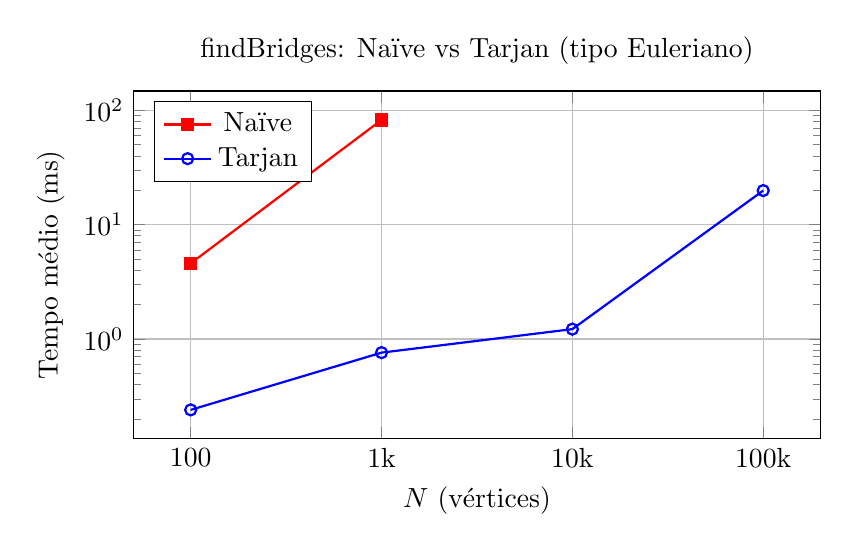
\begin{tikzpicture}
\begin{axis}[
    width=0.85\linewidth, height=6cm,
    xlabel={$N$ (vértices)},
    ylabel={Tempo médio (ms)},
    xmode=log, ymode=log,
    log basis x=10,
    xtick={100,1000,10000,100000},
    xticklabels={100,1k,10k,100k},
    legend pos=north west,
    grid=major,
    title={findBridges: Naïve vs Tarjan (tipo Euleriano)}
]
\addplot[color=red,  mark=square*, thick] coordinates {
    (100,  4.59)
    (1000, 82.40)
};
\addplot[color=blue, mark=o, thick] coordinates {
    (100,    0.24)
    (1000,   0.76)
    (10000,  1.22)
    (100000, 19.87)
};
\legend{Naïve, Tarjan}
\end{axis}
\end{tikzpicture}
\caption{Crescimento do tempo de \texttt{findBridges} em escala log-log.
O Naïve só tem pontos para $N \le 1.000$ (inviável acima disso).}
\label{fig:bridges}
\end{figure}

O Tarjan domina em todos os casos. Em $N=100$ a vantagem é de
$\approx 19{\times}$; em $N=1.000$ chega a $\approx 108{\times}$ no tipo
euleriano (82{,}4~ms contra 0{,}76~ms). Para $N \ge 10.000$ o naïve foi
omitido: a estimativa teórica de $E \cdot (V{+}E) \approx 10^9$ operações
implica vários minutos de execução. O Tarjan resolve o caso de cem mil
vértices em cerca de \textbf{20~ms} --- três ordens de magnitude mais
rápido.

\subsection{Tempo médio do Fleury completo}

\begin{table}[H]
\centering
\caption{Tempo médio do Fleury completo (3 repetições, ms). Em grafos
não-eulerianos o algoritmo aborta na classificação inicial (custo
desprezível). ``--'' indica configuração pulada.}
\label{tab:fleury}
\begin{tabular}{rlrrr}
\toprule
$N$ & Tipo & Arestas & Fleury+Naïve (ms) & Fleury+Tarjan (ms) \\
\midrule
$100$       & Euleriano     & $118$     & $2{,}28$         & $0{,}91$ \\
$100$       & Semi          & $121$     & $0{,}53$         & $0{,}66$ \\
$100$       & Não-Euler.    & $118$     & $0{,}08$         & $0{,}07$ \\
\midrule
$1.000$     & Euleriano     & $1.088$   & $5{,}23$         & $28{,}39$ \\
$1.000$     & Semi          & $1.093$   & $5{,}61$         & $29{,}62$ \\
$1.000$     & Não-Euler.    & $1.092$   & $0{,}58$         & $0{,}55$ \\
\midrule
$10.000$    & Euleriano     & $10.909$  & --               & $20.920{,}13$ \\
$10.000$    & Semi          & $10.884$  & --               & $20.526{,}37$ \\
$10.000$    & Não-Euler.    & $10.916$  & --               & $1{,}65$ \\
\midrule
$100.000$   & Euleriano     & $108.949$ & --               & --\,$^*$ \\
$100.000$   & Semi          & $109.011$ & --               & --\,$^*$ \\
$100.000$   & Não-Euler.    & $108.982$ & --               & --\,$^*$ \\
\bottomrule
\end{tabular}\\[0.4em]
{\small $^*$Em $N=100.000$ a estimativa ultrapassa 30~min:
$E \cdot (V{+}E) \approx 2{,}2 \times 10^{10}$ operações.}
\end{table}

% ====================================================================
\section{Análise dos Resultados}
\label{sec:analise}
% ====================================================================

\subsection{findBridges: Tarjan domina claramente}

Quando o objetivo é \textbf{enumerar todas as pontes}, a vantagem
assintótica do Tarjan se materializa na prática. Uma única DFS de
$O(V{+}E)$ contra $E$ DFS independentes de $O(V{+}E)$ cada. O crescimento
do naïve é claramente quadrático (visível na escala log-log da
Figura~\ref{fig:bridges}); o Tarjan cresce de forma praticamente linear
com o número de arestas.

\subsection{Fleury: resultado contraintuitivo em N = 1.000}

Em $N=1.000$, o Fleury+Naïve (5~ms) foi \textbf{mais rápido} que o
Fleury+Tarjan (28~ms), o que parece contradizer a Tabela~\ref{tab:bridges}.
A explicação está na diferença entre as duas perguntas que o Fleury faz:

\begin{itemize}
    \item \textbf{``Esta aresta específica é ponte?''} --- o naïve usa
          \texttt{isReachable(u,v)}, que para a DFS assim que encontra $v$.
          Em grafos esparsos, $v$ costuma estar a poucos saltos de $u$,
          então a DFS percorre uma fração pequena do grafo.
    \item \textbf{O Tarjan, mesmo só para responder ``sim/não'' sobre uma
          aresta, executa a DFS inteira} para calcular \texttt{low} de todos
          os vértices. O cache versionado ajuda quando o Fleury olha vários
          vizinhos do mesmo vértice \emph{no mesmo passo}, mas a cada
          \texttt{removeEdge} a versão muda e o cache é invalidado.
\end{itemize}

Portanto, a escolha do método certo depende da pergunta:
\begin{itemize}
    \item Para \textbf{enumerar todas as pontes}: Tarjan
          ($O(V{+}E)$ total).
    \item Para \textbf{verificar uma aresta específica por vez} em grafo
          esparso: naïve com \texttt{isReachable} pode ser competitivo.
\end{itemize}

\subsection{Fleury em N = 10.000 e 100.000}

Em $N=10.000$, o Fleury+Tarjan gasta $\approx 21$~s. Isso é coerente com
a estimativa teórica de
$E \cdot (V{+}E) \approx 10.909 \times 21.909 \approx 2 \times 10^8$
operações elementares.

Em $N=100.000$, qualquer variante do Fleury se torna inviável. A detecção
pura de pontes (Tabela~\ref{tab:bridges}) continua em $\approx 20$~ms com
Tarjan, mas o caminho euleriano exige $E$ remoções de aresta com
verificação a cada passo --- algo da ordem de $10^{10}$ operações.
Algoritmos modernos como o de \textbf{Hierholzer} ($O(V{+}E)$)
\cite{hierholzer} seriam a escolha correta para esse tamanho, mas o
enunciado especificou Fleury.

\subsection{Grafos não-eulerianos}

Em todos os tamanhos, ambas as variantes do Fleury terminam em menos de
1~ms para grafos não-eulerianos. O Teorema de Euler é verificado em $O(V)$
(contar graus) e o algoritmo aborta sem percorrer nenhuma aresta. Esse
comportamento é exatamente o esperado.

% ====================================================================
\section{Como Reproduzir os Experimentos}
% ====================================================================

\begin{lstlisting}[language=bash]
# Compilar todos os arquivos
javac -d out src/*.java

# Menu interativo (selecao de tamanho, densidade e tipo)
java -Xss64m -Xmx2g -cp out Main

# Experimentos completos -> gera resultados/experimentos.csv
java -Xss64m -Xmx2g -cp out Main --experiments

# Experimentos modo seguro (pula naive em N >= 10000)
java -Xss64m -Xmx2g -cp out Main --experiments-safe
\end{lstlisting}

O flag \texttt{-Xss64m} aumenta a pilha da JVM e é necessário para o
Tarjan iterativo em grafos grandes. O flag \texttt{-Xmx2g} reserva 2~GB
de heap para os grafos de $100.000$ vértices.

% ====================================================================
\section{Conclusão}
% ====================================================================

Os resultados confirmam a teoria e acrescentam uma nuance prática:

\begin{itemize}
    \item O \textbf{Tarjan} é claramente superior para \textbf{enumerar
          pontes}: até $108{\times}$ mais rápido em $N=1.000$, e único
          método viável a partir de $N=10.000$
          ($\approx 20$~ms para $100.000$ vértices).

    \item No \textbf{Fleury}, o naïve \emph{com} \texttt{isReachable}
          compete com o Tarjan em grafos esparsos de tamanho médio
          ($N=1.000$), pois a terminação antecipada da DFS compensa a
          vantagem assintótica do Tarjan --- resultado contraintuitivo que
          só fica claro ao analisar o custo \emph{real} de cada chamada
          a \texttt{isBridge}.

    \item Para tamanhos $N \ge 10.000$, o Fleury em si se torna o
          gargalo independentemente da estratégia de pontes. O algoritmo
          de Hierholzer ($O(V{+}E)$) seria necessário para escalar além
          disso, mas o enunciado especificou Fleury.
\end{itemize}

% ====================================================================
\begin{thebibliography}{9}
% ====================================================================

\bibitem{tarjan1974}
TARJAN, R. E.
\emph{A note on finding the bridges of a graph}.
Information Processing Letters, v.~2, n.~6, p.~160--161, 1974.
\href{https://doi.org/10.1016/0020-0190(74)90003-9}{doi:10.1016/0020-0190(74)90003-9}.

\bibitem{cormen}
CORMEN, T. H.; LEISERSON, C. E.; RIVEST, R. L.; STEIN, C.
\emph{Introduction to Algorithms}. 3.~ed. MIT Press, 2009.

\bibitem{euler1736}
EULER, L.
\emph{Solutio problematis ad geometriam situs pertinentis}.
Commentarii Academiae Scientiarum Petropolitanae, 1741.

\bibitem{fleury}
FLEURY, M.
\emph{Deux problèmes de géométrie de situation}.
Journal de Mathématiques Élémentaires, 2\textsuperscript{e} série, v.~2,
p.~257--261, 1883.

\bibitem{hierholzer}
HIERHOLZER, C.; WIENER, C.
\emph{Über die Möglichkeit, einen Linienzug ohne Wiederholung und ohne
Unterbrechung zu umfahren}.
Mathematische Annalen, v.~6, p.~30--32, 1873.

\bibitem{so-tarjan}
STACK OVERFLOW.
\emph{Non-recursive version of Tarjan's algorithm}.
Disponível em:
\url{https://stackoverflow.com/questions/46511682/non-recursive-version-of-tarjans-algorithm}.
Acesso em: abr.~2025.

\bibitem{so-dfs}
STACK OVERFLOW.
\emph{Non-recursive DFS implementation}.
Disponível em:
\url{https://stackoverflow.com/questions/14668530/non-recursive-dfs-implementation}.
Acesso em: abr.~2025.

\end{thebibliography}

\end{document}
